\chapter{Introducción}

La industria florícola enfrenta desafíos significativos relacionados con la conservación y el mantenimiento de la calidad de las flores desde su cultivo hasta su comercialización. En este contexto, las cámaras climáticas se presentan como una solución innovadora y eficaz para asegurar las condiciones óptimas de temperatura, humedad y luz necesarias para preservar la frescura y prolongar la vida útil de las flores. Este proyecto empresarial tiene como objetivo desarrollar y evaluar un sistema de cámaras climáticas especializado en flores, abordando aspectos cruciales como el estudio de mercado, el estudio técnico, el estudio administrativo-legal y el estudio económico.

El estudio de mercado se centrará en analizar la demanda actual y futura de cámaras climáticas en la industria florícola, identificando las necesidades específicas de los productores y comerciantes de flores, así como las tendencias y oportunidades del mercado. Este análisis permitirá definir la viabilidad comercial del proyecto y diseñar estrategias efectivas de penetración y posicionamiento en el mercado.

El estudio técnico evaluará las especificaciones y requerimientos tecnológicos necesarios para el desarrollo de las cámaras climáticas, considerando factores como la ingeniería de diseño, los materiales, la eficiencia energética y la automatización de los sistemas de control ambiental. Además, se realizarán pruebas y simulaciones para garantizar el rendimiento y la fiabilidad de las cámaras en diferentes condiciones operativas.

El estudio administrativo-legal abordará la estructura organizativa y los aspectos jurídicos relacionados con la implementación del proyecto, incluyendo la constitución legal de la empresa, los permisos y licencias necesarios, las normativas ambientales y de seguridad, y la gestión de recursos humanos. Este análisis garantizará el cumplimiento de todas las regulaciones y normativas aplicables, minimizando riesgos legales y administrativos.

El estudio económico, acompañado de una evaluación económica detallada, analizará los costos y beneficios asociados al desarrollo y operación de las cámaras climáticas, proyectando ingresos, gastos, flujos de caja y rentabilidad a corto y largo plazo. Esta evaluación permitirá determinar la viabilidad financiera del proyecto y su potencial de retorno de inversión, proporcionando una base sólida para la toma de decisiones estratégicas.

En resumen, este proyecto empresarial tiene como objetivo ofrecer una solución integral y efectiva para la industria florícola mediante el desarrollo de cámaras climáticas avanzadas, asegurando su viabilidad técnica, comercial, administrativa y económica. Con un enfoque multidisciplinario y un análisis exhaustivo en cada uno de los estudios mencionados, buscamos contribuir al crecimiento sostenible y a la competitividad del sector florícola


\chapter{Estudio de mercado}

El estudio de mercado es esencial para comprender el entorno y tomar decisiones estratégicas en el desarrollo y comercialización de cabinas climatizadas para su aplicación en plantas. Esta introducción da una visión del contexto en el que se realizó la investigación y establece la relevancia de los hallazgos del estudio.

\textbf{La realización de este estudio surge de la necesidad de:}

\begin{itemize}
    \item Evaluar la viabilidad y demanda de las cabinas climatizadas para plantas en el mercado local.
    \item Identificar las necesidades y preferencias de los consumidores interesados en este tipo de productos.
\end{itemize}

\textbf{Objetivo del Estudio de Mercado}

El objetivo específico del estudio de mercado es obtener información sobre el mercado objetivo, identificar el perfil del público interesado y evaluar la relación entre oferta y demanda de las cabinas climatizadas para plantas en la región de Valles Centrales de Oaxaca de Juárez. 

\section{Definición y descripción del producto}

Las cabinas climatizadas para plantas son espacios cerrados diseñados para mantener condiciones específicas de temperatura, radiación UV y humedad. 

\textbf{Características}
\begin{itemize}
    \item Diseño Modular: Las cabinas se fabrican con paneles prefabricados para que se puedan añadir accesorios.
    \item Climatización: Control preciso de la temperatura y humedad mediante sistemas de aire acondicionado y calefacción.
    \item Aislamiento: Paneles con alto aislamiento térmico para mantener condiciones internas estables.
    \item Iluminación Interna: Incorporan sistemas de iluminación para facilitar el trabajo en su interior.
\end{itemize}

\textbf{Ventajas}
\begin{itemize}
    \item Espacio Personalizado: Se pueden instalar en áreas específicas sin necesidad de climatizar todo el lugar.
    \item Ahorro de Energía: Eficiencia energética al mantener condiciones óptimas sin desperdiciar recursos.
    \item Comodidad y seguridad: Protección contra condiciones climáticas extremas.
    \item Flexibilidad: Adaptación a diferentes usos, como oficinas, zonas de almacenamiento o salas de control.
\end{itemize}

\textbf{Desventajas}
\begin{itemize}
    \item Costo Inicial: La inversión inicial puede ser alta debido a la tecnología y materiales utilizados.
    \item Mantenimiento: Requieren mantenimiento para asegurar su funcionamiento óptimo, aunque este no sea frecuente.
    \item Dependencia de Energía: Necesitan fuentes de energía para la climatización.
\end{itemize}

\subsection{Análisis de la materia prima }
La materia prima para la elaboración de las cabinas climatizadas para el desarrollo de las plantas cuenta de una diversidad de componentes, en su mayoría de naturaleza electrónica, a continuación, se presenta un listado de materiales a usar y su costo comercial. 

\begin{table}[H]
\centering
\caption{Lista de materiales}
\begin{tabular}{|p{4cm}|p{3cm}|p{3cm}|p{3cm}|}
\hline
\textbf{Materia prima utilizada}
&\textbf{Costo por unidad} &\textbf{Unidades utilizadas} &\textbf{Costo total}\\
\hline
Hoja de madera 1.5m x 2m & 950 & 1 &950\\
\hline
Acrílico & 750 & 1 & 750\\
\hline
Bisagras & 75 & 2 & 150\\
\hline
Tornillos & & & 200\\
\hline
Pegamento & 120 & 1 &120\\
\hline
ESP32 & 200 &1 &200\\
\hline
ESP32 CAM &200&1 &200\\
\hline
DHT11&60 &x &60x\\
\hline
Relés & 40 & x & 40x \\
\hline
Motor & 600 & 1 &600\\
\hline
Display Oled 128x64 & 90&1&90\\
\hline
RTC&135&1&135\\
\hline
Puente H&55&1&55\\
\hline
Ultrasónico&35&2&70\\
\hline
Celda peltier&425&x&425x\\
\hline
Buzzer&35&1&35\\
\hline
\end{tabular}
\label{tabla:piezasSoporteEstabilizador}
\end{table}

\section{Análisis de la demanda}
Estas cabinas forman parte de una línea especifica de productos relacionados con la jardinería. Los consumidores que estén interesados en el cultivo de las plantas en interiores o espacios limitados pueden buscar dichas cabinas como una solución práctica.

\section{Definición del mercado}

El mercado meta es la población de las principales ciudades y destinos turísticos del estado de Oaxaca, de sexo indistinto que perciban salarios medios a altos y que tengan como pasatiempo o trabajo el cuidado de plantas.

Este grupo incluye a los amantes de la jardinería, propietarios de viviendas con espacio para plantas y personas interesadas en plantas de interior.
Las empresas de jardinería, viveros y tiendas especializadas pueden ser parte del mercado. Estos negocios pueden adquirir cabinas para ofrecer a sus clientes o utilizarlas para el cultivo de plantas en sus instalaciones.

Oaxaca es un destino turístico popular, y las cabinas para el cuidado de las plantas podrían ser atractivas para hoteles y alojamientos que deseen proporcionar un ambiente verde y relajante para sus huéspedes.

\subsection{Tamaño de la muestra}
Para calcular el tamaño de la muestra necesaria para obtener resultados certeros, se utiliza la siguiente fórmula:

\[
n = \frac{{\sigma^2 Upq}}{{e^2 (U - 1) + \sigma^2 pq}}
\]

Donde:

U = 1496300 (población de Oaxaca con ingresos mayores al mínimo)
{\sigma = 1.96} \textit{(Coeficiente de confianza)}

\[
p = 0.5, q=0.5, e = 0.05
\]

Teniendo como resultado 

\[
n = 384 \textit{ respuestas}
\]

El tamaño del universo U     se tomó de la población que no se encuentra en algún estado de pobreza en la población del estado, siendo la fuente principal el CONEVAL \cite{Coneval}.

\begin{figure}[H]
    \centering	
    \includegraphics[width=.8\textwidth]{img/Empresa/Población 2020.jpg} 
    \caption{Medición de pobreza 2020}
\label{fig:MedicionPobreza2020}
\end{figure}

\subsection{Proyección de la demanda }
Los datos analizados para poder proyectar la demanda contienen información recopilada del INEGI \cite{Censo2020} \cite{INEGIOaxaca} y el CONEVAL. Además, algunos de los datos principales recabados por la encuesta se encuentran en anexos.

\begin{table}[h]
\centering
\begin{tabular}{|c|c|c|}
\hline
\textbf{AÑO} & \textbf{X} & \textbf{Y (Millones de habitantes)} \\
\hline
1900 & 1 & 0.9 \\
1910 & 2 & 1 \\
1921 & 3 & 1 \\
1930 & 4 & 1.1 \\
1940 & 5 & 1.2 \\
1950 & 6 & 1.4 \\
1960 & 7 & 1.7 \\
1970 & 8 & 2 \\
1980 & 9 & 2.4 \\
1990 & 10 & 3 \\
2000 & 11 & 3.4 \\
2010 & 12 & 3.8 \\
2020 & 13 & 4.1 \\
\hline
\end{tabular}
\caption{Tabla de población del estado de Oaxaca (INEGI)}
\label{tab:tablaPoblacionOaxaca}
\end{table}

\begin{figure}[H]
    \centering	
    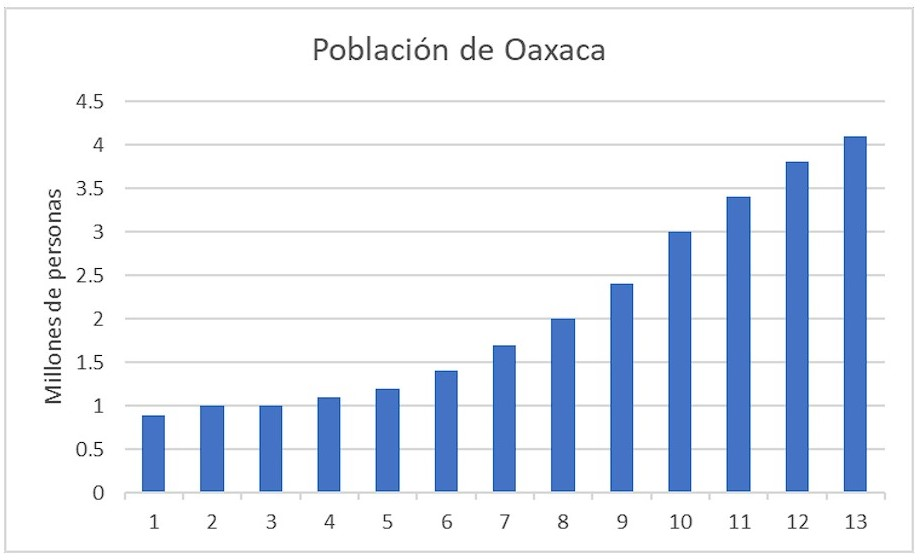
\includegraphics[width=.8\textwidth]{img/Empresa/GraficaPoblacion.jpg} 
    \caption{Gráfica de la población}
\label{fig:GraficaPoblacionOaxaca}
\end{figure}

Debido a que los datos del adquiridos por el CONEVAL empiezan desde el 2008 se extrapolaron datos en los intervalos necesarios para tener una mejor resolución de los datos.

\begin{table}[h]
\centering
\begin{tabular}{|c|c|c|}
\hline
\textbf{AÑO} & \textbf{X} & \textbf{Y (Millones de habitantes)} \\
\hline
2000 & 1 & 3.4 \\
2002 & 2 & 3.48 \\
2004 & 3 & 3.56 \\
2006 & 4 & 3.64 \\
2008 & 5 & 3.72 \\
2010 & 6 & 3.8 \\
2012 & 7 & 3.86 \\
2014 & 8 & 3.92 \\
2016 & 9 & 3.98 \\
2018 & 10 & 4.04 \\
2020 & 11 & 4.1 \\
2022 & 12 & 4.19 \\
2024 & 13 & 4.26 \\
2026 & 14 & 4.33 \\
2028 & 15 & 4.40 \\
2030 & 16 & 4.47 \\
\hline
\end{tabular}
\caption{Tabla de población extrapolada}
\label{tab:PoblacionExtrapolada}
\end{table}

\begin{figure}[H]
    \centering	
    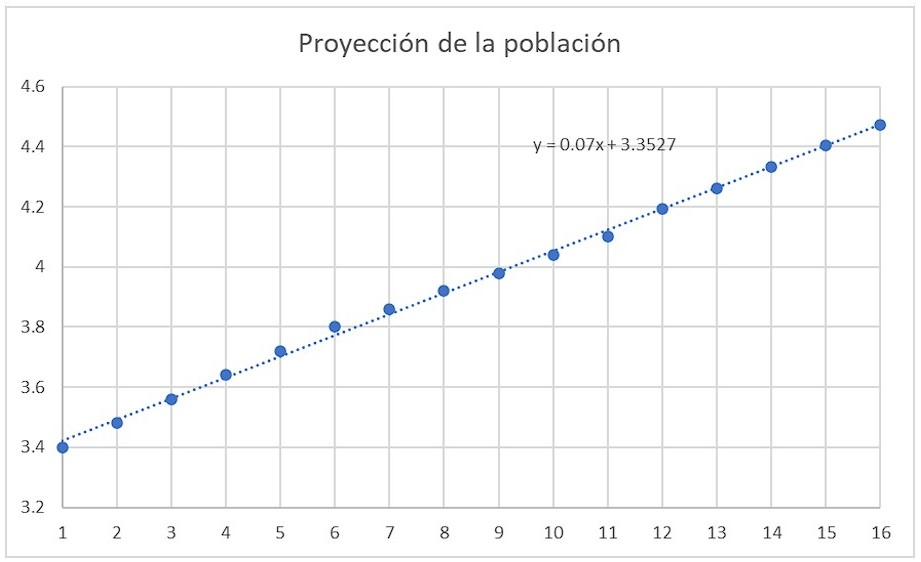
\includegraphics[width=.8\textwidth]{img/Empresa/PosibleCrecimientoPoblacional.jpg} 
    \caption{Gráfica de posible crecimiento poblacional}
\label{fig:GraficaPoblacionOaxacaAprox}
\end{figure}

Sin embargo, según los últimos reportes de la CONEVAL, los índices de pobreza y pobreza extrema en el estado rondan el 60\%, sin embargo, no estar en situación de pobreza no es suficiente para poder adquirir nuestro producto, así que nos enfocamos en la parte de la población que no se encuentra en ningún tipo de pobreza ni vulnerabilidad. Según el último reporte de la CONEVAL, esta parte de la población representa el 23.5\% (tercera columna).
Además, el análisis de la encuesta realizada arroja que el 40\% de las personas encuestadas tienen problemas al cuidar sus plantas, delimitando de mejor manera el mercado objetivo (cuarta columna).

\begin{table}[h!]
\centering
\begin{tabular}{|c|c|c|c|c|}
\hline
\textbf{AÑO} & \textbf{X} & \textbf{Millones de habitantes} & \textbf{No pobres ni vulnerables} & \textbf{Posibles consumidores} \\
\hline
2008 & 1 & 3.72 & 0.7 & 0.28 \\
2010 & 2 & 3.8 & 0.76 & 0.30 \\
2012 & 3 & 3.86 & 0.76 & 0.31 \\
2014 & 4 & 3.92 & 0.8 & 0.32 \\
2016 & 5 & 3.98 & 0.9 & 0.36 \\
2018 & 6 & 4.04 & 0.96 & 0.38 \\
2020 & 7 & 4.1 & 0.96 & 0.39 \\
2022 & 8 & 4.19 & 1.04 & 0.42 \\
2024 & 9 & 4.26 & 1.09 & 0.44 \\
2026 & 10 & 4.33 & 1.15 & 0.46 \\
2028 & 11 & 4.4 & 1.21 & 0.48 \\
2030 & 12 & 4.47 & 1.27 & 0.51 \\
\hline
\end{tabular}
\caption{Evolución de la población y posibles consumidores}
\label{tab:my_label}
\end{table}


\begin{figure}[H]
    \centering	
    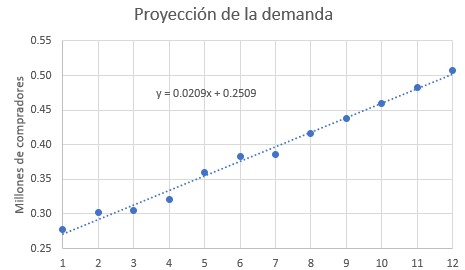
\includegraphics[width=.8\textwidth]{img/Empresa/ProyeccionDemanda.jpg} 
    \caption{Gráfica de proyección de la demanda}
\label{fig:GraficaProyeccionDemanda}
\end{figure}

En conclusión, según la proyección de la demanda, se esperan vender 280,000 unidades para el primer año.

\section{Análisis de la oferta }

En estas cabinas hechas para el ámbito de la jardinería se debe evaluar el marcado y competencia para determinar la demanda y viabilidad del proyecto

\textbf{Evaluación del mercado}
El mercado de cabinas automatizadas para el cuidado de plantas es un nicho emergente en México. Estas cabinas ofrecen soluciones innovadoras para el cultivo y mantenimiento de plantas en entornos controlados. Pese a su potencial, enfrentan desafíos significativos por la falta de productores locales y servicios de mantenimiento. En este informe, exploraremos en detalle la situación actual del mercado y las posibles estrategias para su desarrollo.


\textbf{Oferta actual}

\textbf{Equipos semi automatizados en línea:}

Existen opciones de cabinas semi automatizadas disponibles en páginas de internet. Estos equipos ofrecen funciones básicas como iluminación programable, riego automático y control de temperatura. Sin embargo, su alcance es limitado y no cumplen con los estándares de una cabina completamente automatizada.
La mayoría de estos equipos son importados y no se fabrican localmente en México.

\textbf{Ausencia de productores locales:}

A pesar de la creciente demanda, no existen productores especializados en la fabricación de cabinas para el cuidado de plantas en México.
La falta de producción local dificulta la disponibilidad, personalización y adaptación a las necesidades específicas del mercado mexicano.

\textbf{Demanda y oportunidades}

\textbf{Creciente interés en la jardinería interior:}

La tendencia hacia la jardinería interior y la decoración con plantas ha aumentado en los últimos años. Cada día se realizan 3 mil millones de búsquedas en Google. El 20\% de esas búsquedas son inéditas. En promedio se realizan 135,000 búsquedas al mes con enfoque en plantas, basados en datos de answer the public.

\begin{figure}[H]
    \centering	
    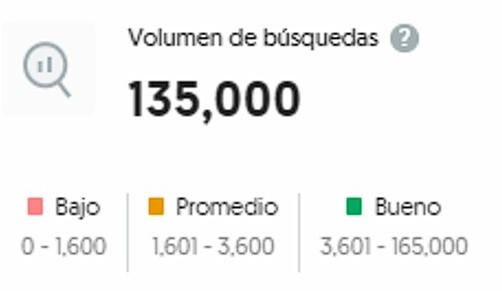
\includegraphics[width=.4\textwidth]{img/Empresa/VolumenBusquedas.jpg} 
    \caption{Volumen de búsquedas sobre jardinería en internet}
\label{fig:GraficaProyeccionDemanda}
\end{figure}

En general las personas buscan soluciones prácticas y estéticas para mantener sus plantas en espacios reducidos.

\textbf{Mercado potencial:}

El mercado objetivo incluye a entusiastas de la jardinería, propietarios de viviendas, oficinas, restaurantes y hoteles.
La conciencia ambiental y la búsqueda de soluciones sostenibles también impulsan la demanda.

\textbf{Necesidad de mantenimiento y reparación:}

Las cabinas automatizadas requieren mantenimiento regular para garantizar su funcionamiento óptimo.
La falta de servicios de mantenimiento y reparación es una barrera para la adopción masiva.

\textbf{Estrategias y propuestas}

\textbf{Fomentar la producción local:}

Se deben incentivar iniciativas para desarrollar productores locales que fabriquen cabinas de alta calidad.
Esto incluye la capacitación en diseño, fabricación y control de calidad.

\textbf{Alianzas con instituciones educativas y centros de investigación:}

Colaborar con universidades y centros de investigación para impulsar la innovación en el diseño y fabricación de cabinas.
Establecer programas de investigación y desarrollo para mejorar la tecnología y la eficiencia.

\textbf{Servicios de mantenimiento y reparación:}

Fomentar la creación de servicios especializados en mantenimiento y reparación de cabinas automatizadas.
Capacitar técnicos y establecer redes de soporte para atender las necesidades de los usuarios.

\textbf{Desafíos del mercado}

\textbf{Escasez de productores locales:}

Uno de los principales desafíos es la falta de productores especializados en la fabricación de cabinas para el cuidado de plantas en México.
La mayoría de las opciones disponibles son importadas, lo que dificulta la adaptación a las necesidades específicas del mercado local.

\textbf{Complejidad tecnológica:}

Las cabinas automatizadas requieren tecnología avanzada para controlar factores como la iluminación, la humedad y la temperatura.
La falta de conocimiento técnico y experiencia en la fabricación de estas cabinas puede ser un obstáculo.

\textbf{Costos iniciales y percepción del valor:}

Las cabinas automatizadas pueden tener un costo inicial significativo.
Convencer a los consumidores de su valor a largo plazo y beneficios sostenibles es un desafío importante.

El mercado de cabinas para el cuidado de plantas en México está en una etapa de crecimiento y transformación. Aprovechar las oportunidades y superar los desafíos requerirá una colaboración activa entre los diferentes actores involucrados. La inversión en investigación, desarrollo y educación será clave para satisfacer la creciente demanda de soluciones sostenibles en la jardinería interior.

\section{Análisis de precio}

El siguiente análisis de precios tiene como finalidad realizar la investigación necesaria para conocer los precios actuales en el mercado local, estatal e internacionalmente, ya que hoy se puede conseguir un producto similar por varios medios. Para esta investigación se estudiaron a los diferentes competidores y se realizó el análisis para establecer precios y lineamientos en los diferentes intermediarios que se establecieron.  

Para recabar la información de la competencia se investigó a la competencia y se realizó el siguiente análisis de datos. El análisis de precios siguió una técnica parecida la presentada en \cite{Gonzalez}. 

\textbf{Precios de los productores a los intermediarios:}

Para estudiar a la competencia que ofrezca un producto similar dentro de la zona que distribuiremos, no hay establecimiento al que se pueda estudiar, pero no solo hay competidores locales a los que se investigó, también hay competidores nacionales e internacionales con los que se puede comparar, ya que, aunque no se encuentran como tal en la localidad, si son parte de la competencia al poder vender y entregar un producto similar en la misma localidad donde estamos. 
El producto que ofrecen es directamente entre vendedor y comprador, a diferencia de nosotros, siendo los primeros en el territorio local podemos fijar el precio a nuestros clientes intermediarios, para analizar primero los precios de la competencia entre vendedor y comprador final. 

\textbf{Precios de los productores a los clientes finales:}

El precio que ofrece directamente AliExpress \cite{AliExpress} a los clientes finales es

\begin{table}[h!]
\centering
\begin{tabular}{|l|l|l|r|}
\hline
\multicolumn{2}{|c|}{\textbf{PRODUCTO}} & \textbf{TAMAÑO} & \textbf{PRECIO} \\ \hline
\multirow{2}{*}{Vendedor A} & Cámara climática, Tipo A & 120*165*115 & \$3442 \\
                            & Cámara climática, Tipo B & 130*170*125 & \$16088 \\ \hline
\multirow{2}{*}{Vendedor B} & Cámara climática, Tipo A & 120*165*115 & \$3613 \\
                            & Cámara climática, Tipo B & 130*170*125 & \$14455 \\ \hline
\multirow{2}{*}{Vendedor C} & Cámara climática, Tipo A & 120*165*115 & \$3322 \\
                            & Cámara climática, Tipo B & 130*170*125 & \$23388 \\ \hline
\end{tabular}
\caption{Precio asignado directamente al comprador final}
\end{table}


Las características de este análisis son que para poder obtener el producto se deben esperar de una semana a un mes para que llegue la máquina. El costo de envió es adicional y este puede variar dependiendo del año. Para poder encontrar alguna relación el cliente tiene que pedir información al vendedor y esperar aún más tiempo para el envío lo que le generara un gasto extra. Además, para poder operar la maquina no tiene un servicio que te la instalen, lo tiene que realizar el comprador con un manual y unos videos adicionales en algunos casos, de lo contrario, se debe buscar una persona capacitada para operarla adecuadamente, lo que le generaría más gastos adicionales al comprador.

En cuanto a la investigación realizada, las empresas que venden este producto, nacional o internacionalmente, son directas entre vendedor y comprador, nosotros al no tener una empresa cercana para poder fijar un precio para un intermediario se fijará uno, ya que tendremos intermediarios para expandirse rápidamente. Si llega una empresa se podrá reunir si se desea para fijar precios que beneficie a ambos.


\textbf{Precios del proyecto}


\begin{table}[h!]
\centering
\begin{adjustbox}{width=\textwidth}
\begin{tabular}{|l|c|c|p{5cm}|p{5cm}|c|c|}
\hline
\multicolumn{3}{|c|}{} & \multicolumn{2}{c|}{\textbf{Características}} & \multicolumn{2}{c|}{\textbf{Precio al cliente final}} \\ \cline{4-7} 
\multicolumn{3}{|c|}{\multirow{-2}{*}{\textbf{Producto}}} & \textbf{Competencia} & \textbf{Proyecto} & \textbf{Competencia} & \textbf{Proyecto} \\ \hline
\multirow{3}{*}{Vendedor A Modelo A,B} & \multicolumn{2}{c|}{120*165*115} & Tiene cámara de humedad, control de temperatura y ambiente de simulación. &  & \$3442 &  \\ \cline{2-7} 
 & \multicolumn{2}{c|}{125*165*120} &  & Tiene una cámara mediante la cual se puede controlar la temperatura, la presión, la luminosidad además detectar si cierto tipo de plantas están en deterioro. & \$6000 &  \\ \cline{2-7} 
 & \multicolumn{2}{c|}{130*170*125} &  &  & \$16088 &  \\ \hline
\multirow{2}{*}{Vendedor B Modelo A,B} & \multicolumn{2}{c|}{120*165*115} & Rango amplio de variación de temperatura, variabilidad de presiones &  & \$3613 &  \\ \cline{2-7} 
 & \multicolumn{2}{c|}{130*170*125} &  &  & \$14455 &  \\ \hline
\multirow{2}{*}{Vendedor C Modelo A,B} & \multicolumn{2}{c|}{120*165*115} & Variabilidad de temperaturas, así como a ritmo constante &  & \$3322 &  \\ \cline{2-7} 
 & \multicolumn{2}{c|}{130*170*125} &  &  & \$23388 &  \\ \hline
\end{tabular}
\end{adjustbox}
\caption{Comparativa de precios a clientes finales entre la competencia y el proyecto \cite{AliExpress}}
\label{tab:comparativa}
\end{table}



Después de asignar los precios entre los intermediarios que se puedan colocar en el local de la empresa donde se ofrecerá el mismo producto con todas sus características, ofreciendo promociones dependiendo del paquete as adquirir o el servicio a comprar. 

\begin{table}[h!]
\centering
\begin{adjustbox}{width=\textwidth}
\begin{tabular}{|l|l|l|l|l|}
\hline
\textbf{Producto} & \textbf{Tamaño} & \multicolumn{2}{l|}{\textbf{Precio}} & \textbf{Margen de utilidad} \\
\cline{3-4}
 & & \textbf{Intermediarios} & \textbf{Comprador final} & \\
\hline
Cámara climática & 125*165*120 & \$5600 & \$6000 & \$400 \\
\hline
\end{tabular}
\end{adjustbox}
\caption{Precios del proyecto asignados a los intermediarios y comprador final}
\end{table}


Respecto a los márgenes de utilidad para los intermediarios, no se tienen definidos dentro del estado solo se podrían comprar al menos que entrare un vendedor en el mismo ambiente, de ser así se volvería hacer un análisis de precio comparándolo con la competencia para poder realizar un ajuste si fuera necesario.

\section{Comercialización de los productos }

Una comercialización es la actividad que permite al productor hacer llegar un bien o servicio al consumidor con los beneficios de tiempo y lugar, para esto existen diferentes canales de distribución. Para la elección de estos canales es importante seleccionar un canal de distribución que permita llegar de manera eficiente a los potenciales clientes y maximice la visibilidad y accesibilidad del producto. Tomando en cuenta las características que nuestro producto y el mercado objetivo que queremos lograr los principales canales de distribución son los siguientes:

\textbf{Venta Directa a través de showrooms o exposiciones especializadas:}

Este canal permite mostrar físicamente las cabinas climatizadas, lo que facilita a los clientes potenciales ver y experimentar el producto en persona. Además, al tratarse de un producto especializado, la interacción directa con representantes de ventas capacitados puede ser crucial para explicar las características y ventajas del producto.

\textbf{Distribución a través de empresas de construcción o ingeniería:}

Las empresas de construcción o ingeniería pueden ser aliados estratégicos para la comercialización de las cabinas climatizadas, especialmente si se utilizan en proyectos de construcción o remodelación de espacios específicos donde se requieran condiciones controladas. Estas empresas pueden integrar las cabinas como parte de sus soluciones para ofrecer a sus clientes finales.

\textbf{Venta a través de distribuidores especializados en equipamiento industrial o agrícola:}

Los distribuidores especializados en equipamiento industrial o agrícola ya tienen una red establecida de clientes que podrían estar interesados en las cabinas climatizadas para sus actividades comerciales. Estos distribuidores pueden proporcionar una cobertura geográfica más amplia y facilitar el acceso al producto en diferentes áreas de la ciudad de Oaxaca y sus alrededores.
Comercialización en Línea a través de Plataformas de Comercio 

\textbf{Electrónico especializadas:}

La venta en línea a través de plataformas especializadas en equipamiento industrial o agrícola puede ampliar significativamente el alcance del producto más allá de la ciudad de Oaxaca. Este canal permite llegar a clientes potenciales en todo el país e incluso a nivel internacional, aprovechando el potencial de expansión del mercado.

\section{Conclusiones del estudio de mercado}

